% LaTeX source for ``การเรียนรู้ของเครื่องสำหรับเคมีควอนตัม (Machine Learning for Quantum Chemistry)''
% Copyright (c) 2022 รังสิมันต์ เกษแก้ว (Rangsiman Ketkaew).

% License: Creative Commons Attribution-NonCommercial-NoDerivatives 4.0 International (CC BY-NC-ND 4.0)
% https://creativecommons.org/licenses/by-nc-nd/4.0/

\chapter{ชุดข้อมูลทางเคมี}
\label{ch:chem_dataset}

ชุดข้อมูลคือการเก็บข้อมูลให้อยู่ในรูปแบบที่สามารถแบ่งประเภทของข้อมูลในชุดข้อมูลได้ โดยส่วนใหญ่แล้วเรามักจะเก็บข้อมูลในรูปแบบของตาราง
โดยตารางของชุดข้อมูลนั้นอาจจะมีหลายคอลัมน์ก็ได้ โดยแต่ละคอลัมน์จะแสดงถึงตัวแปรเฉพาะของข้อมูล ข้อมูลนั้นเป็นสิ่งที่สำคัญและเป็นองค์ประกอบ%
ที่ขาดไม่ได้เลยในการสร้างโมเดลปัญญาประดิษฐ์ ซึ่งการที่เรามีข้อมูลมหาศาลในทุกวันนี้ก็อาจจะเรียกได้ว่าเป็นสาเหตุหลักที่ทำให้เกิดการเรียนรู้ของเครื่อง%
ขึ้นมาได้ ชุดข้อมูลถือได้ว่าเป็นหัวใจสำคัญของการเรียนรู้ของเครื่องเลยก็ว่าได้ ถ้าหากเรามีชุดข้อมูลดี เราก็สามารถสร้าง Feature Input Vector 
ให้กับโมเดลที่เราต้องการจะฝึกสอนได้ แต่ถ้าหากชุดข้อมูลของเราไม่ได้ สิ่งที่ตามมาก็คือโมเดลที่ถูกฝึกสอนออกมานั้นก็จะมีประสิทธิภาพในการทำนายที่ต่ำมาก
(Garbage In, Garbage Out) 

%--------------------------
\section{ชุดข้อมูล}
\label{sec:dataset}
%--------------------------

\begin{figure}[H]
    \centering
    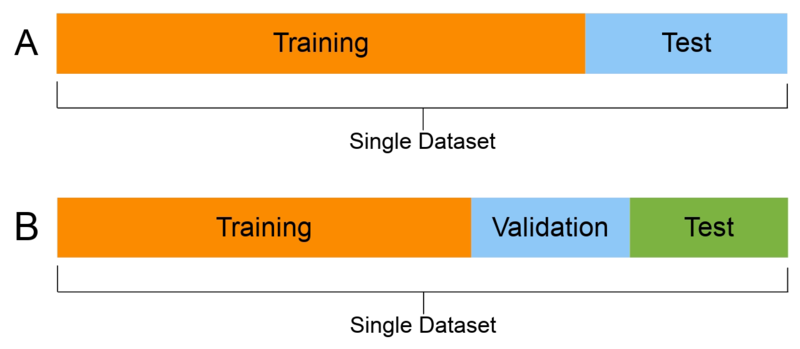
\includegraphics[width=0.7\linewidth]{fig/dataset.png}
    \caption{ตัวอย่างชุดข้อมูลแบบ 2 มิติ โดยมี Feature คือ Score, Attempts, Qualify (เครดิตภาพ: w3resource.com)}
    \label{fig:dataset}
\end{figure}

เรามาทำความรู้จักกับชุดข้อมูลกันมากกว่านี้ดีกว่าครับ เริ่มจากเราต้องทำความเข้าใจมิติของชุดข้อมูล (Dimensionality of Dataset) กันก่อน
ซึ่งมิติของชุดข้อมูลก็จะมีตั้งแต่ 1 มิติ, 2 มิติ, 3 มิติ, 4 มิติ หรือสูงมากกว่านั้นก็ได้ ให้ลองนึกถึง Tensor ซึ่งเราสามารถเพิ่มจำนวนมิติของข้อมูลได้
สำหรับกรณีที่ชุดข้อมูลมี 1 มิตินั้นจะง่ายที่สุดเพราะเราจะมองว่าชุดข้อมูลแบบนี้เป็นเวกเตอร์ก็ได้ ชุดข้อมูล 1 มิติก็คือข้อมูลที่มีหลายแถวแต่มีแค่ 1 หลัก 
หรือจะเป็นชุดข้อมูลที่มีเพียงแค่ 1 แถวแต่มีหลายหลักก็ได้ สำหรับชุดข้อมูลแบบ 2 มิตินั้นให้เปรียบเทียบกับตาราง ซึ่งตารางประกอบไปด้วยแถวและหลัก
โดยเราจะมองว่าตารางนั้นจริง ๆ แล้วก็คือเมทริกซ์ก็ได้ ซึ่งชุดข้อมูล 2D ประกอบด้วยมิติของแถว (Row) และมิติของหลักหรือคอลัมน์ (Column) 
เมื่อนำจำนวนของแถวคูณกับจำนวนของหลัก (Row x Column) จะได้ขนาดของชุดข้อมูล (Size) ซึ่งสอดคล้องกับขนาดของเมทริกซ์ เช่น 
ชุดข้อมูลขนาด 125 x 50 หมายความว่าชุดข้อมูลนี้คือชุดข้อมูลขนาด 2 มิติ ที่มีจำนวนข้อมูลทั้งหมด 125 แถว แต่ละแถวมี 50 หลัก 
สำหรับชุดข้อมูล 3 มิติ ก็จะมีอีก 1 มิติเพิ่มเข้ามานอกเหนือจากแถวกับหลักซึ่งจะถูกเรียกว่าอะไรนั้นก็ขึ้นอยู่กับว่าข้อมูลนั้นเป็นข้อมูลประเภทไหน 
เพราะว่าบางครั้งเราก็ไม่ได้ใช้คำว่าแถวกับหลัก เช่น ถ้าเป็นชุดข้อมูลรูปภาพ ก็จะใช้ ความสูง x ความกว้าง x ความลึก (Height x Width x Depth) 
ซึ่งก็สามารถเรียงสลับได้
\idxth{ชุดข้อมูล!มิติของชุดข้อมูล}
\idxen{Dataset!Dimensionality of Dataset}

%--------------------------
\section{ประเภทและการแบ่งชุดข้อมูล}
\label{sec:split_dataset}
\idxth{ชุดข้อมูล!ประเภทของชุดข้อมูล}
\idxen{Dataset!Type of Dataset}
\idxth{ชุดข้อมูล!การแบ่งชุดข้อมูล}
\idxen{Dataset!Dataset Splitting}
%--------------------------

ชุดข้อมูลที่ใช้ใน ML นั้นโดยทั่วไปแล้วมักจะมีอยู่ 2 ประเภทคือชุดข้อมูลสำหรับการฝึกสอน (Training Set) และชุดข้อมูลสำหรับการทดสอบ 
(Test Set) ซึ่งวัตถุประสงค์ของชุดข้อมูลทั้งสองประเภทนี้ก็ตรงตัวเลยก็คือ Training Set จะถูกนำมาใช้ในการฝึกสอนโมเดล ส่วน Test Set 
จะถูกเก็บไว้ใช้ในการทดสอบโมเดลหรือการทำนายคำตอบที่โมเดลถูกสอนมา (Prediction) อย่างไรก็ตาม การฝึกสอนโมเดลโดยการใช้ Train Set 
ทั้งหมดนั้นมักจะทำให้เกิดความโน้มเอียง (Bias) ที่เกิดขึ้นจากชุดข้อมูลและส่งผลให้เกิด Biased ในขั้นตอน Prediction ด้วย เพราะป้องกันเหตุการณ์%
ดังกล่าวและทำให้เกิด Bias น้อยที่สุด เรามักจะทำการแบ่ง (Split) ชุดข้อมูลฝึกสอนให้เป็นชุดข้อมูลสำหรับการฝึกสอนจริง ๆ (Actual Training 
Set) และชุดข้อมูลสำหรับการตรวจสอบและยืนยันความถูกต้องซึ่งเรียกอีกอย่างว่า Validation Set

\begin{figure}[H]
    \centering
    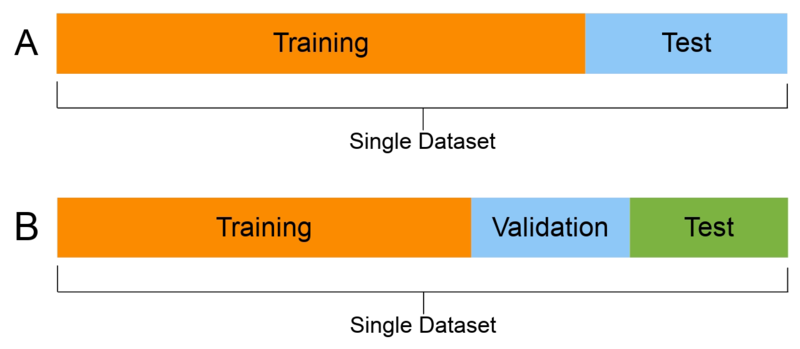
\includegraphics[width=0.8\linewidth]{fig/dataset_splitting.png}
    \caption{การแบ่งชุดข้อมูลทั้งหมดออกเป็น (A) Training Set และ Test Set และ (B) Training Set, Validation Set และ 
    Test Set (เครดิตภาพ: Wikimedia Commons)}
    \label{fig:dataset_splitting}
\end{figure}

ภาพที่ \ref{fig:dataset_splitting} แสดงสัดส่วนแบบคร่าว ๆ ในการแบ่งชุดข้อมูลหลักออกเป็น Training Set และ Test Set 
และแสดงการแบ่งชุดข้อมูล Training Set อีกครั้งให้เป็น Actual Training Set ที่จะถูกนำไปใช้ในการฝึกสอนโมเดลจริง ๆ และ Validation 
Set ที่จะถูกนำมาทดสอบโมเดลเพื่อเป็นการหยั่งเชิงความสามารถของโมเดลก่อนที่จะนำไปใช้ทำนายค่าของเอาต์พุตของข้อมูลใน Test Set%
\footnote{โดยทั่วไปแล้วหลาย ๆ คนมักจะทำการแบ่งชุดข้อมูลโดยใช้อัตราส่วนคือ 80\% (สำหรับ Training Set) และ 20\% (สำหรับ Test
Set) ตามหลักการของ Pareto ซึ่งสามารถอ่านเพิ่มเติมได้ที่ \url{https://en.wikipedia.org/wiki/Pareto_principle}}

แล้วขั้นตอนการลด Bias นั่นมันเกิดขึ้นได้อย่างไร คำตอบก็คือในการแบ่งข้อมูลออกมาเป็น Validation Set (เช่นแบ่งออกมา 20\% จากทั้งหมด)
โดยทำการสุ่มเลือกบางส่วนของข้อมูลออกมา ซึ่งถ้าหากเราทำวนไปแบบนี้ไปเรื่อย ๆ เราจะเรียกว่าเป็นการทำ Validation แบบข้ามไปมาทั่วทั้ง 
Training Set ซึ่งเมื่อเรานำ Training Set แต่ละชุดไปฝึกสอนโมเดล เราจะได้ประสิทธิภาพของโมเดลแบบเฉลี่ย เปรียบเสมือนเป็นการเกลี่ย% 
หาความเท่ากันของข้อมูลนั่นเอง (กระจายออกไปให้เสมอกัน) ท้ายที่สุดแล้วถ้าเราแบ่งชุดข้อมูลตามที่ได้อธิบายมา เราจะมีอัตราส่วนของชุดข้อมูล%
ย่อย ๆ แต่ละประเภท ดังนี้

\begin{itemize}
    \item Training: 80\%
    \begin{itemize}
        \item Actual Training Set: 60\%
        
        \item Cross Validation: 20\%
    \end{itemize}
    
    \item Testing: 20\%
\end{itemize}

%--------------------------
\section{การสร้างชุดข้อมูล}
\label{sec:create_dataset}
\idxth{ชุดข้อมูล!การสร้างชุดข้อมูล}
%--------------------------

ขั้นตอนการสร้างชุดข้อมูลประกอบไปด้วย 3 ขั้นหลักดังนี้

\paragraph{1. รวบรวมข้อมูล (Collect)} สิ่งแรกที่เราจะทำในการมองหา Dataset ก็คือแหล่งข้อมูลที่เราสามารถนำข้อมูลมาใช้ได้ ถ้าหากแหล่งข้อมูลไม่น่าเชื่อถือ
เราก็มักจะได้ชุดข้อมูลที่ไม่น่าเชื่อถือและอาจจะมีข้อผิดพลาดในชุดข้อมูลด้วยเช่นกัน เช่น ข้อมูลที่สร้างขึ้นมา (ข้อมูลปลอมหรือ Fake) 

\paragraph{2. ประมวลผลข้อมูลก่อน (Preprocess)} หลักการสำคัญข้อหนึ่งของวิทยาศาสตร์เชิงข้อมูลเลยก็คือทำความสะอาดชุดข้อมูล (Data 
Cleaning) รวมไปถึงการทราบที่มาที่ไปและการทำความเข้าใจชุดข้อมูล เราต้องถามตัวเองก่อนว่าชุดข้อมูลที่เราสนใจนั้นเคยถูกใช้มาก่อนหน้านี้หรือยัง 
ถ้าหากว่ายัง เราควรจะต้องตั้งข้อสังเกตหรือสมมติฐานไว้ก่อนว่าชุดข้อมูลชุดนี้อาจจะมีข้อมูลที่ผิดปกติซ่อนอยู่ได้ หรืออาจจะมีข้อมูลที่ไม่ครบถ้วนขาดหายไป 
เราสามารถทำการประมวลผลชุดข้อมูลก่อนนำไปใช้งานจริงได้โดยการดูที่คุณภาพของ Features รวมไปถึง Bias ภายในชุดข้อมูล บางชุดข้อมูลมี 
Features เยอะมากแต่ว่ามี Bias เยอะมาก ๆ กับ Features เพียงแค่ 2-3 Features นอกจากนี้แล้วปริมาณของชุดข้อมูลก็มีผลด้วย 
เพราะว่าถ้าหากเรามีปริมาณข้อมูลที่น้อยเกินไปก็อาจจะเกิดปัญหา Overfitting ได้ในภายหลัง

\paragraph{3. การทำคำอธิบายประกอบ (Annotate)} หลังจากทำความสะอาดข้อมูลเสร็จเรียบร้อยแล้วสิ่งที่เราควรจะต้องในลำดับต่อไปคือ Annotate 
นั่นคือเป็นการทำให้มั่นใจว่าข้อมูลของเรานั้นมันสามารถนำไปใช้ในการสอนเครื่องจักรเข้าใจได้ กล่าวง่าย ๆ คือทำให้คอมพิวเตอร์สามารถเรียนรู้จากข้อมูลได้
นั่นก็เพราะว่าเครื่องจักรไม่ได้เข้าใจข้อมูลเหมือนอย่างที่มนุษย์เข้าใจ ดังนั้นเราควรจะต้องทำการเพิ่มคำอธิบายเชิงดิจิตอลให้กับข้อมู,นั่นก็คือการทำ Labeling

%--------------------------
\section{ปริภูมิเคมี}
\label{sec:chem_space}
\idxboth{ปริภูมิเคมี}{Chemical Space}
%--------------------------

ปริภูมิเคมี (Chemical space)\autocite{kirkpatrick2004}

%--------------------------
\section{ชุดข้อมูลเคมีควอนตัม}
\label{ssec:step_create_qm_dataset}
\idxth{ชุดข้อมูล!การสร้างชุดข้อมูลเคมีควอนตัม}
\idxen{Dataset!Create Dataset}
%--------------------------

%--------------------------
\section{ชุดข้อมูลมาตรฐาน}
\label{sec:std_dataset}
\idxth{ชุดข้อมูล!ชุดข้อมูลมาตรฐาน}
\idxen{Dataset!Standard Dataset}
%--------------------------

QM9 เป็นหนึ่งใน Dataset ที่ได้รับความนิยมมากในสายงานวิจัยเคมีควอนตัม โดยเฉพาะงานวิจัยทางด้าน ML ซึ่งถูกใช้อย่างแพร่หลายตั้งแต่ปี ค.ศ. 
2014 เป็นต้นมา\autocite{ruddigkeit2012,ramakrishnan2014} โดยบทความวิจัยแรกที่ได้รับการตีพิมพ์นั้นรายงานค่าความแม่นยำและ%
ความผิดพลาดของโมเดล ML ว่าไม่เกิน 10 kcal/mol ซึ่งถือว่าคลาดเคลื่อนเยอะมาก ๆ และต่อมาได้มีการพัฒนาระเบียบวิธีวิจัยรวมไปถึงโมเดล ML 
และ Descriptor ใหม่ ๆ จนทำให้ในปัจจุบันนั้นนักวิจัยสามารถที่จะทำนายหรือพยากรณ์ค่าพลังงานของโมเลกุลทางเคมีอินทรีย์ขนาดเล็กได้แม่นยำมาก%
โดยมีค่าความคลาดเคลื่อนประมาณ 1 kcal/mol หรือต่ำกว่านั้น ซึ่งเป็นค่าที่เรียกว่า \textit{ค่าความถูกต้องทางเคมี (Chemical Accuracy)} 
หรือเทียบเท่ากับค่าความคลาดเคลื่อนของเครื่องมือทดลองทางเคมี ซึ่งค่าดังกล่าวเป็นค่ามาตรฐานที่ต่ำที่สุดที่เทคนิคทางการทดลองสามารถวัดได้
โดยถ้าหากว่าต่ำไปกว่านี้แล้วเทคนิคต่าง ๆ จะไม่สามารถให้ความคลาดเคลื่อนที่แม่นยำได้อีกต่อไป

QM9 ประกอบไปด้วยข้อมูลคุณสมบัติอิเล็กทรอนิกส์ของโมเลกุลมากถึง 134,000 โมเลกุล โดยทุกโมเลกุลมีธาตุพื้นฐานเป็นองค์ประกอบ ประกอบไปด้วย 
คาร์บอน (C), ไนโตรเจน, (N), ออกซิเจน (O), ไฮโดรเจน (H), และฟลูออรีน (F) โดย Feature หลักของ QM9 ก็จะมีพิกัดคาร์ทีเซียนของ%
อะตอมทุกอะตอมในโมเลกุลซึ่งได้มาจากการคำนวณการปรับโครงสร้าง (Geometry Optimization) ด้วยระเบียบวิธี B3LYP/6-31G(2df,p) 
และนอกจากนี้ยังมีค่า Label หรือค่าที่ไว้ใช้ในการเปรียบเทียบการพยากรณ์ดังแสดงในตารางที่ \ref{tab:qm9_feature}%
\footnote{โมเดล ML ที่เหมาะสมสำหรับการฝึกสอนด้วย QM9 นั้นจะต้องไม่ขึ้นกับ Translation, Rotation และ Permutation}

\begin{table}[H]
    \centering
    \caption{ข้อมูล Feature ของชุดข้อมูล QM9}
    \label{tab:qm9_feature}
    \small
    \begin{tabular}{llll}\toprule
    \textbf{ดัชนี} &\textbf{ชื่อ} &\textbf{หน่วย} &\textbf{คำอธิบาย} \\\midrule
    0 &index &- &Consecutive, 1-based integer identifier of molecule \\
    1 &A &GHz &Rotational constant A \\
    2 &B &GHz &Rotational constant B \\
    3 &C &GHz &Rotational constant C \\
    4 &mu &Debye &Dipole moment \\
    5 &alpha &Bohr$^3$ &Isotropic polarizability \\
    6 &homo &Hartree &พลังงานของ Highest occupied molecular orbital (HOMO) \\
    7 &lumo &Hartree &พลังงานของ Lowest unoccupied molecular orbital (LUMO) \\
    8 &gap &Hartree &Gap (พลังงานระหว่าง LUMO and HOMO) \\
    9 &r2 &Bohr$^2$ &Electronic spatial extent \\
    10 &zpve &Hartree &Zero point vibrational energy \\
    11 &U0 &Hartree &Internal energy at 0 K \\
    12 &U &Hartree &Internal energy at 298.15 K \\
    13 &H &Hartree &Enthalpy at 298.15 K \\
    14 &G &Hartree &Free energy at 298.15 K \\
    15 &Cv &cal/(mol K) &Heat capacity at 298.15 K \\
    \bottomrule
    \end{tabular}
\end{table}

ชุดข้อมูล QM9 สามารถดาวน์โหลดมาใช้งานได้ฟรีจากเว็บไซต์ \url{http://quantum-machine.org/datasets/} โดยจะมีข้อมูลพิกัดคาร์ทีเซียน
(Cartesian Coordinates), คุณลักษณะ (Features), และค่าพลังงานซึ่งเป็น Target ของเรา คราวนี้เราลองมาดูโค้ดสำหรับการใช้งาน 
QM9 โดยใช้ Python ตามด้านล่างนี้เลย

\noindent ทำการเรียกใช้ไลบรารี่และอ่านไฟล์ของชุดข้อมูล
\begin{lstlisting}[style=MyPython]
# Import libraries
import ase.io as aio
import pandas as pd

# Read qm9.csv
qm9_data = pd.read_csv('./qm9.csv', index_col=0)
\end{lstlisting}

\noindent เราสามารถใช้คำสั่งด้านล่างในการแสดง Target ได้

\begin{lstlisting}[style=MyPython]
target = qm9_data['u0'] * 627.5096080305927 # we convert it from Hartree to kcal/mol
print(target)

# OUTPUT
0         -25400.917498
40       -121896.331092
80       -146555.740566
120      -122481.233425
160      -168344.348805
              ...      
119800   -242900.012196
119840   -230424.279698
119880   -266202.856340
119920   -252980.566249
119960   -288738.466448
Name: u0, Length: 3000, dtype: float64
\end{lstlisting}

\noindent อ่านพิกัดคาร์ทีเซียนของโมเลกุล

\begin{lstlisting}[style=MyPython]
# We read xyz coorinates of all the molecules with ase aio.read tool
ase_mols = [aio.read('data/qm9/qm9_xyz/' + mol + '.xyz') for mol in qm9_data.mol_id]
\end{lstlisting}

\noindent ตรวจสอบขนาดของโมเลกุลที่ใหญ่ที่สุดในชุดข้อมูล

\begin{lstlisting}[style=MyPython]
# Check the size of molecules in the dataset
size=[]
for mol in ase_mols:
    num = len(mol.get_atomic_numbers())
    size.append(num)
max(size) #maximum size of the molecule in the dataset

# OUTPUT
27
\end{lstlisting}

โดยโค้ดด้านบนที่เราใช้สำหรับการโหลดชุดข้อมูล QM9 นั้นเราจะนำไปใช้ต่อในบทที่ \ref{sec:pred_tot_ener} สำหรับการทำนายพลังงานรวม%
ของโมเลกุลของชุดข้อมูล QM9 \ref{ssec:pred_spec_ir}

นอกจาก QM9 แล้วยังมีชุดข้อมูลอื่น ๆ ที่นักวิจัยมักจะนำมาใช้ในการฝึกสอนโมเดลและทำวิจัย เช่น 

\begin{itemize}
    \item QM7\autocite{blum2009,rupp2012a}
    
    \item QM7b\autocite{blum2009,montavon2013}
    
    \item QM8\autocite{ruddigkeit2012,ramakrishnan2015}
    
    \item ISO17\autocite{schutt2017,schutt2017a,ramakrishnan2014}
\end{itemize}

\noindent ซึ่งก็จะมี Label สำหรับวัตถุประสงค์ในการฝึกสอนโมเดลในการเพิ่มความสามารถการพยากรณ์คุณสมบัติเคมีของโมเลกุลที่ต่างกันออกไป 
โดยชุดข้อมูลที่กล่าวมาทั้งหมดนั้นสามารถดาวน์โหลดได้ฟรีจากเว็บไซต์ \url{http://quantum-machine.org/datasets} เช่นกัน

%--------------------------
\section{การวิเคราะห์ชุดข้อมูล}
\label{sec:dataset_analysis}
\idxth{ชุดข้อมูล!การวิเคราะห์ชุดข้อมูล}
\idxen{Dataset!Dataset Analysis}
%--------------------------

หลังจากที่เราเลือกชุดข้อมูลที่ต้องการนำมาศึกษาแล้ว ลำดับต่อไปคือการคำนวณ Feature Vector ซึ่งจะถูกนำไปใช้ในการฝึกสอนโมเดล ML ต่อไป
โดย Feature ที่ผู้เขียนจะยกตัวอย่างให้ได้ศึกษานั้นก็จะเป็น Feature ที่ใช้ Descriptor แบบง่ายนั่นก็คือ Coulomb Matrix (CM)
ผู้เขียนจะยังคงใช้ชุดข้อมูล QM9 และใช้โค้ดต่อไปนี้ในการคำนวณ CM ของโมเลกุลตัวอย่างเพียงแค่ 3,000 โมเลกุลเท่านั้น

\begin{lstlisting}[style=MyPython]
import numpy as np
from qml.representations import * 

cm = []
size = 27 # Maximum size of molecule in the set

# Runs for loop over every molecule in the database
for structure in ase_mols: 
    # ASE prints atomic numbers 
    atomic_numbers = structure.get_atomic_numbers() 
    # ASE prints coordinates
    coordinates=structure.get_positions() 
    cm1 = generate_coulomb_matrix(atomic_numbers,
    # CM representation is saved into cm1
    coordinates, size = size, sorting="row-norm") 
    # All CM representations are added into one variable
    cm.append(cm1) 

# Transforms cm into numpy array
cm = np.array(cm) 
# Check size of cm
print(cm.shape)

# OUTPUT
(3000, 378)
\end{lstlisting}

หลังจากที่เราคำนวณ CM ของโมเลกุลในชุดข้อมูลเสร็จเรียบร้อยแล้ว สิ่งที่หลายคนทำในละดับต่อไปก็คือสร้างโมเดลแล้วนำ Feature Vector 
หรืออินพุตที่ได้ไปใช้ในการฝึกสอนโมเดลทันทีเลย ซึ่งการทำแบบนี้นั้นจริง ๆ แล้วไม่เหมาะสมเท่าไหร่นัก นั่นก็เพราะว่าเราควรจะต้องทำความเข้าใจ 
Feature ที่เราคำนวณออกมาก่อนโดยทำการวิเคราะห์เพื่อดูลักษณะการกระจายตัวหรือการจัดกลุ่มซึ่งสามารถบอกแนวโน้มรวมไปถึง Bias ได้

เราสามารถใช้เทคนิค Unsupervised ML แบบง่าย ๆ ที่ไม่ซับซ้อน เช่น Principal Component Analysis (PCA) ซึ่งเป็นวิธีที่ลดจำนวนมิติ 
(Dimensionality Reduction) ของข้อมูลให้อยู่ในรูปขององค์ประกอบเชิงตั้งฉาก (Orthogonal Component) ที่อธิบายปริมาณของความแปรปรวน
(Variance) ที่มากที่สุด หรือจะใช้วิธี t-distributed Stochastic Neighbor Embedding (t-SNE) ซึ่งเป็นวิธีที่สามารถแสดงข้อมูลที่มีมิติสูง ๆ 
(Highd-dimensional Data) ได้เช่นเดียวกัน\autocite{JMLR:v9:vandermaaten08a,belkina2019} โดยจะทำเปลี่ยนความเหมือนกันระหว่าง%
ข้อมูลสองชุดให้เป็นความน่าจะเป็นร่วม (Joint Probability) แล้วทำการปรับค่า Kullback-Leibler Divergence ระหว่างความน่าจะเป็นร่วม%
ของข้อมูลที่อยู่ในมิติต่ำและมิติสูงให้น้อยที่สุด (Minimization)\footnote{เทคนิค t-SNE ถูกพัฒนาต่อมาจากเทคนิค SNE ซึ่งแรกเริ่มนั้นพัฒนาโดย
Geoffrey Hinton และ Sam Roweis แห่งมหาวิทยาลัยโทรอนโต ประเทศแคนาดา\autocite{NIPS2002_6150ccc6} หลังจากนั้น Laurens 
van der Maaten ได้ทำการเพิ่ม t-distributed เข้าไป} ซึ่งเราสามารถใช้ทั้ง PCA และ t-SNE ในการวิเคราะห์เพื่อดูลักษณะหรืออธิบายง่าย ๆ 
คือดู \enquote{\textit{รูปร่างหน้าตา}} ของ CM ของทั้ง 3,000 โมเลกุลที่คำนวณออกมาได้โดยใช้โค้ดต่อไปนี้
\idxen{t-distributed Stochastic Neighbor Embedding}

\noindent สร้างโมเดล t-SNE
\begin{lstlisting}[style=MyPython]
import sklearn

tsne_cm = sklearn.manifold.TSNE(n_components=2)
tsne_cm_data = tsne_cm.fit_transform(cm)
\end{lstlisting}

\noindent สร้างโมเดล PCA
\begin{lstlisting}[style=MyPython]
pca_cm = sklearn.decomposition.PCA(n_components=2)
pca_cm_data = pca_cm.fit_transform(cm)
\end{lstlisting}

\noindent พลอตกราฟค่าที่ได้จากการ Fit ข้อมูล
\begin{lstlisting}[style=MyPython]
import matplotlib.pyplot as plt

fig, axs = plt.subplots(1,2,figsize=(15,9))
axs[0].set_title('Principal Components')
axs[1].set_title('t-SNE')

plot1 = axs[0].scatter(pca_cm_data[:, 0], pca_cm_data[:, 1], c=target, cmap='jet', s=1)
plot2 = axs[1].scatter(tsne_cm_data[:, 0], tsne_cm_data[:, 1], c=target, cmap='jet', s=1)

cbar = fig.colorbar(plot2, ax=axs);
cbar.set_label('Internal energy at 0 K [kcal/mol]')
plt.show()
\end{lstlisting}

\noindent พลอตที่ได้จะเป็นแบบนี้ โดยข้อมูลแต่ละจุดนั้นจะถูกไฮไลต์ด้วยสีที่มีสเกลแตกต่างกันไปซึ่งแสดงค่าของพลังงานภายในของโมเลกุล

\begin{figure}[H]
    \centering
    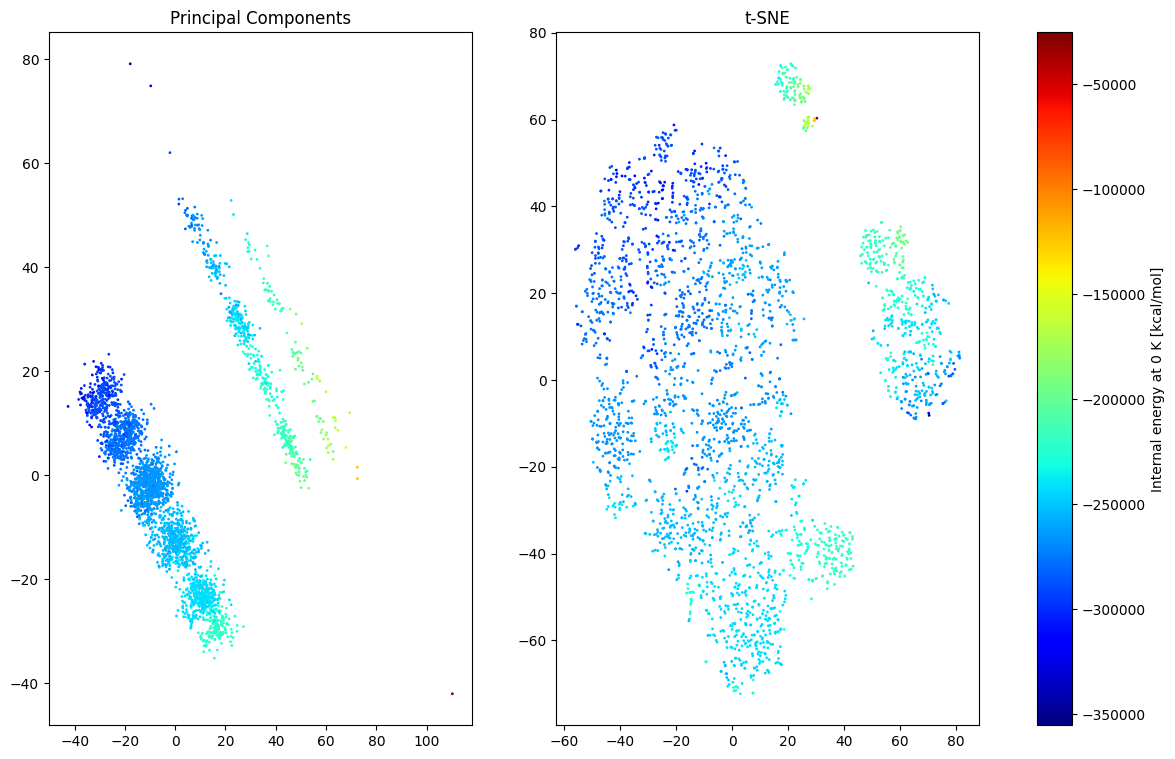
\includegraphics[width=\linewidth]{fig/cm_pca_tsne.png}
    \caption{การกระจายตัวของ Coulomb Matrix Feature ที่ถูกลดจำนวนมิติให้เหลือเพียงแค่ 2 มิติ (Principal Component = 2)}
    \label{fig:cm_pca_tsne}
\end{figure}
